% This is samplepaper.tex, a sample chapter demonstrating the
% LLNCS macro package for Springer Computer Science proceedings;
% Version 2.20 of 2017/10/04
%
%\documentclass[runningheads]{llncs}
\documentclass[sn-mathphys-num]{sn-jnl}
%
\usepackage{graphicx}
% Used for displaying a sample figure. If possible, figure files should
% be included in EPS format.
%
% If you use the hyperref package, please uncomment the following line
% to display URLs in blue roman font according to Springer's eBook style:
% \renewcommand\UrlFont{\color{blue}\rmfamily}

% My packages
\usepackage{amsmath} 
\usepackage{algorithm}
\usepackage{algpseudocode}
\usepackage[numbers]{natbib} % CItation in appearance order
\usepackage{subcaption}
\usepackage{orcidlink}
\usepackage{pdflscape}
\usepackage{booktabs}
\usepackage{float}
%\usepackage{mdframed}
%\usepackage{hyperref}
\usepackage{tabularx}

\usepackage{orcidlink}


% To eliminate hyphens
\tolerance=9000
\emergencystretch=0pt
\hyphenpenalty=10000
\hbadness=10000
\frenchspacing


\begin{document}
%\title{Optimization of Surgical Operating Room Utilization Through Job Shop Scheduling Techniques: A Real-World Case Study in Puerto Montt}
%\title{Applying N×M Job Shop Scheduling Models to Surgical Suite Management for Lead Time and Throughput Optimization}
%\title{Operational Optimization of Hospital Operating Rooms Using Manufacturing Scheduling Approaches: Evidence from a Chilean Hospital}
\title{From Job Shops to Operating Rooms: A Throughput-Oriented Scheduling Framework for Surgical Block Optimization\thanks{Supported by Pepe, Hospital de Puerto Montt, Chile}}
%
%\titlerunning{Optimizing the No-Show Problem}
% If the paper title is too long for the running head, you can set
% an abbreviated paper title here
%
\author*[1,2]{\fnm{Andrés} \sur{Leiva-Araos}}%\orcidlink{0000-0002-2480-3022}}
\email{andresleiva@udd.cl}
%\equalcont{\small These authors contributed equally to this work.}
%&\equalcont{\small These authors contributed equally to this work.}

\author[3]{\fnm{Pablo} \sur{Aguilera}}
\email{pablo.aguilera.t@mail.pucv.cl}

\author[3,4]{\fnm{Bady} \sur{Gana}}
\email{bady.gana@pucv.cl}

\author*[3,4]{\fnm{Marcelo} \sur{Becerra}}
\email{marcelo.becerra@pucv.cl}

\affil[1]{\orgdiv{Instituto Data Science}, \orgname{Universidad del Desarrollo}, \orgaddress{\street{Av. La Plaza 680}, \city{Las Condes}, \postcode{7610658}, \state{RM}, \country{Chile}}}

\affil*[2]{\orgdiv{Department of Computing}, \orgname{University of North Florida}, \orgaddress{\street{1 UNF Dr.}, \city{Jacksonville}, \postcode{32246}, \state{FL}, \country{USA}}}

\affil[3]{\orgdiv{Escuela de Ingeniería Informática}, \orgname{Pontificia Universidad Católica de Valparaíso}, \orgaddress{\street{Av. Brasil 2241}, \city{Valparaiso}, \postcode{2362807}, \state{Valparaíso}, \country{Chile}}}

\affil[4]{\orgdiv{Center for Interdisciplinary Research in Biomedicine, Biotechnology and Well-Being (CID3B)}, \orgname{Pontificia Universidad Católica de Valparaíso}, \orgaddress{\street{Av. Brasil 2950}, \city{Valparaiso}, \postcode{2362807}, \state{Valparaíso}, \country{Chile}}}


\abstract{
    Lorem ipsum dolor sit amet, consectetur adipiscing elit. Mauris turpis erat, lobortis nec maximus vel, finibus sed est. Curabitur nec purus tincidunt, pellentesque purus et, suscipit ligula. Praesent eu efficitur augue. Fusce nec lacinia orci, ut suscipit felis. Curabitur vel mauris ut justo facilisis sodales sit amet in magna. In at mollis sapien. Vestibulum ante ipsum primis in faucibus orci luctus et ultrices posuere cubilia curae; Duis ac massa ex. Vivamus nibh purus, luctus id lacus nec, rutrum cursus felis. Nunc turpis lacus, facilisis sit amet finibus eget, laoreet in nulla. Donec sollicitudin ex eu semper pretium. Mauris porttitor cursus magna, et hendrerit orci elementum vel. Cras porta, orci feugiat ultricies lacinia, risus diam iaculis tortor, ut porta ipsum diam sit amet risus. In hac habitasse platea dictumst. Morbi malesuada auctor mauris, vehicula elementum eros finibus vestibulum. Vivamus pretium sem vitae arcu interdum, ut semper eros aliquet. Praesent ornare consectetur felis, posuere consequat ligula venenatis suscipit. Etiam felis risus, bibendum ac nibh quis, sagittis lacinia ipsum. Praesent rhoncus metus sit amet turpis elementum aliquet. Phasellus congue dolor sit amet nulla viverra auctor. Proin consequat turpis auctor odio convallis vehicula. Phasellus ac dignissim enim, quis condimentum felis. Etiam molestie mollis imperdiet. Maecenas vehicula metus sed ligula rhoncus consequat. Phasellus eu diam volutpat, viverra felis eu, interdum tortor. Mauris venenatis nulla urna, ut tempus sem aliquet quis. Vivamus gravida dictum malesuada. Maecenas quis ante bibendum, mollis ipsum ac, commodo nisi. Orci varius natoque penatibus et magnis dis parturient montes, nascetur ridiculus mus. Cras vel dui sem. Phasellus id urna lacinia, consequat tortor eget, consequat nisl. Quisque laoreet ac nulla vitae porta. Vivamus rutrum purus a nulla laoreet sollicitudin. Donec nec nunc tempus, tincidunt elit vel, varius felis. 
}
\keywords{Operating Room Scheduling, Job Shop Scheduling, Throughput Optimization, Lead Time Reduction, Healthcare Operations Management}

%
\maketitle  
%
% ================================================================
\section{Introduction}\label{sec:intro}

Efficient surgical care delivery is a cornerstone of hospital performance,
yet managing operating room (OR) capacity remains one of the most complex
operational challenges in healthcare systems worldwide. The simultaneous
presence of scheduled elective procedures and unscheduled urgent cases
creates inherent tension between productivity and responsiveness, a problem
that is particularly acute in public hospitals operating under persistent
resource constraints. This study addresses that challenge through a
discrete-event simulation model parameterized with real clinical-operational
data from a Chilean public hospital, providing empirical evidence on the
comparative performance of simple dispatching rules under mixed elective-urgent
demand conditions.

\subsection{The Operating Room Scheduling Problem and its Impacts}

The OR represents one of the most resource-intensive and
financially consequential components of hospital infrastructure. Inpatient
stays involving surgical procedures account for a disproportionate share of
total hospital costs \cite{mcdermott2021overview}, with ORs estimated to generate
over 50\% of hospital revenues while simultaneously contributing more than
25\% of total operating expenses in many healthcare systems \cite{macario2010does}.
In hospitals that concurrently manage scheduled elective caseloads alongside
unscheduled urgent surgical demand, operational decisions regarding case
prioritization and OR assignment have a direct and measurable impact on key
performance indicators, including resource utilization, patient waiting times,
surgical throughput, overtime costs, and case cancellation rates
\cite{may2011surgical,lamiri2008stochastic}. The coexistence of both demand types introduces a
structural trade-off between maximizing elective productivity and sustaining
responsive capacity for emergency contingencies, a tension further compounded
by the stochastic nature of surgical procedure durations and the
unpredictability of urgent arrival processes \cite{gerchak1996reservation,may2011surgical}.

In healthcare systems where surgical demand persistently exceeds installed
capacity, a condition prevalent across the public hospital networks of many
low- and middle-income countries \cite{meara2015global}, this trade-off acquires
heightened operational significance. The COVID-19 pandemic further amplified
pre-existing structural deficits: across Latin America and the Caribbean, the
large-scale suspension of elective surgical activity generated unprecedented
backlogs that placed extraordinary strain on recovery capacity well into the
post-pandemic period \cite{campos2024examining}. In Chile, institutional assessments
have documented persistent and significant gaps between installed OR capacity
and effective surgical output, with considerable inter-facility variability
across the public health network \cite{aguilar2022como,de2020uso}.
Studies have reported marked variation in elective OR occupancy rates during
the 2018--2021 period \cite{barahona2023estimacion}, while analyses of surgical case
cancellations have identified substantial opportunities for performance
improvement through better utilization of existing resources, without
necessarily requiring additional infrastructure investment \cite{catalan2022suspensiones}.
These operational gaps coexist with challenges in clinical information
management quality and completeness, where the availability of structured,
high-quality operational data constitutes a necessary prerequisite for
evidence-based monitoring and continuous improvement of surgical processes
\cite{avendano2025chile,MINSAL2023}.

\subsection{Opportunities to Explore}

Despite the extensive international literature on OR planning and scheduling
\cite{avendano2025chile,guerriero2011operational,hulshof2012taxonomic}, empirical evidence evaluating
operational policies under real-world mixed elective-urgent demand conditions
in Latin American public hospitals remains limited. The vast majority of
existing studies are grounded in high-income country settings with
substantially different governance structures, funding mechanisms, and health
information infrastructure from those characteristic of the Chilean public
sector \cite{zhu2019operating}. Three specific gaps in the literature motivate the
present work. First, there is a scarcity of simulation models directly
parameterized with real clinical-operational data from Chilean public hospitals
that simultaneously capture the coexistence of elective and urgent surgical
demand with their respective temporal dynamics. Second, systematic comparative
evaluations of simple, interpretable dispatching rules are lacking; these
represent the most operationally feasible policies in resource-constrained
health information environments, and their benchmarking under parameters
representative of actual system operation remains an open empirical question.
Third, there is a need for empirically grounded baseline benchmarks against
which more sophisticated approaches such as stochastic optimization or
metaheuristics can be rigorously evaluated prior to adoption, given that the
implementation of such methods in public hospital settings entails additional
barriers of computational complexity and operational transparency \cite{rios2011just,brailsford2016healthcare}.


%***AGREGAR LOCALIZACIÓN DE PUERTO MONTT.
\subsection{Project Goals}

Motivated by this context, the present study develops a minute-by-minute
discrete-event simulation (DES) model parameterized with real
clinical-operational records from Hospital Puerto Montt Dr.\ Eduardo Schütz
Schroeder, and uses it to compare simple dispatching rules (FIFO, SPT, and
LPT) combined with two OR assignment modalities (sequential and alternating).
DES was selected as the methodological framework given its demonstrated
suitability for evaluating operational policies in systems characterized by
stochastic demand, multiple interacting resources, and complex temporal
dynamics, where analytical tractability is limited and controlled
experimentation on the real system is infeasible
\cite{gunal2010discrete,jun1999application,vazquez2021discrete}.
Hospital Puerto Montt is a high-complexity referral center belonging to the
Servicio de Salud del Reloncaví, operating 12 surgical theaters across 21
specialties with an annual surgical volume of approximately 7{,}000
interventions. The dataset used comprises 28{,}464 surgical intervention
records spanning January 2020 through December 2023, including scheduled
procedures, emergency cases, and unscheduled surgeries, with detailed
timestamps, ICD-10 diagnoses, specialty classifications, and team composition.

The contributions of this work are:
\begin{itemize}
  \item To develop and document a minute-by-minute discrete-event simulator
  for a mixed elective-urgent OR system, directly parameterized with real data
  from a Chilean public hospital, incorporating uncertainty in surgical
  durations (modeled by ICD-10 code via maximum likelihood estimation and
  goodness-of-fit selection) and urgent arrivals modeled as a non-homogeneous
  Poisson process with Bayesian inference via Metropolis-Hastings.
  \item To compare six strategies resulting from combining three dispatching
  rules (FIFO, SPT, and LPT) with two assignment modalities (sequential and
  alternating), evaluated over 30 independent replications with 95\%
  confidence intervals, under a base configuration coherent with the
  hospital's 24/7 operational structure.
  \item To provide an extensible simulation framework that supports the
  evaluation of additional operational policies, including dedicated OR
  assignment, differentiated time windows, and capacity reservation
  mechanisms, thereby establishing an empirical foundation for future
  extensions toward integrated perioperative models.
\end{itemize}

The remainder of this paper is organized as follows...



\section{Literature Review}

    To ensure a comprehensive and systematic approach to the literature review, we developed a Systematic Topic Review framework inspired by the methodology proposed in \cite{gana2024leveraging}. The process began with the extraction of relevant articles from PubMed and Scopus using the query in Table \ref{tab:query}, which produced a total of 1,122 documents.

    
    \begin{table}[ht]
        \centering
        \caption{Literature search query statement.}
        \label{tab:query}
        \vspace{5pt} % Espacio entre el caption y la tabla
        \begin{tabular}{@{}|c|@{}}
            \hline
            \\
            \textit{{\color{purple}(TITLE-ABS-KEY (}\;"no*show"{\color{purple}\;)}} \\
            \textit{{\color{purple}OR TITLE-ABS-KEY (}\;"non*attendance"{\color{purple}\;)}} \\
            \textit{{\color{purple}AND TITLE-ABS-KEY (}\;"medicine" OR "healthcare" OR "health care"{\color{purple}\;)}} \\
            \\
            \hline
        \end{tabular}
    \end{table}
    

    
    \textcolor{blue}{These documents were then processed through the workflow depicted in Fig. \ref{fig:STR-workflow}. The key steps included query extraction, data preprocessing, and the application of BERTopic, which leveraged an embedding model (BAAI/bge-latrge-en-v1.5) and dimensionality reduction for clustering and topic summarization. To enhance relevance, we filtered the dataset to include only papers published within the last 10 years, reducing the corpus to 755 documents. The results of this process were further refined through an expert medical review, which identified and validated the most relevant topics for inclusion in the literature review. This combined computational and expert-driven approach ensured the selection of relevant and impactful topics, providing a solid foundation for the systematic review. Based on the BERTopic process, we identified 25 distinct topics, of which medical experts selected 5 as the most relevant. Within these 5 primary topics, we curated 105 papers, which were selected based on their citation level and recency to form the core of our literature review. This core analysis was further enriched with insights from a secondary group of 12 additional topics, comprising 321 articles, which were analyzed to extract specific case studies related to no-show phenomena. Table \ref{tab:topics_relevance} presents a detailed list of primary and secondary topics, highlighting their respective contributions to our systematic review. The column “Count” indicates the number of documents grouped under each topic.}

    \begin{figure}[h]
        \centering
        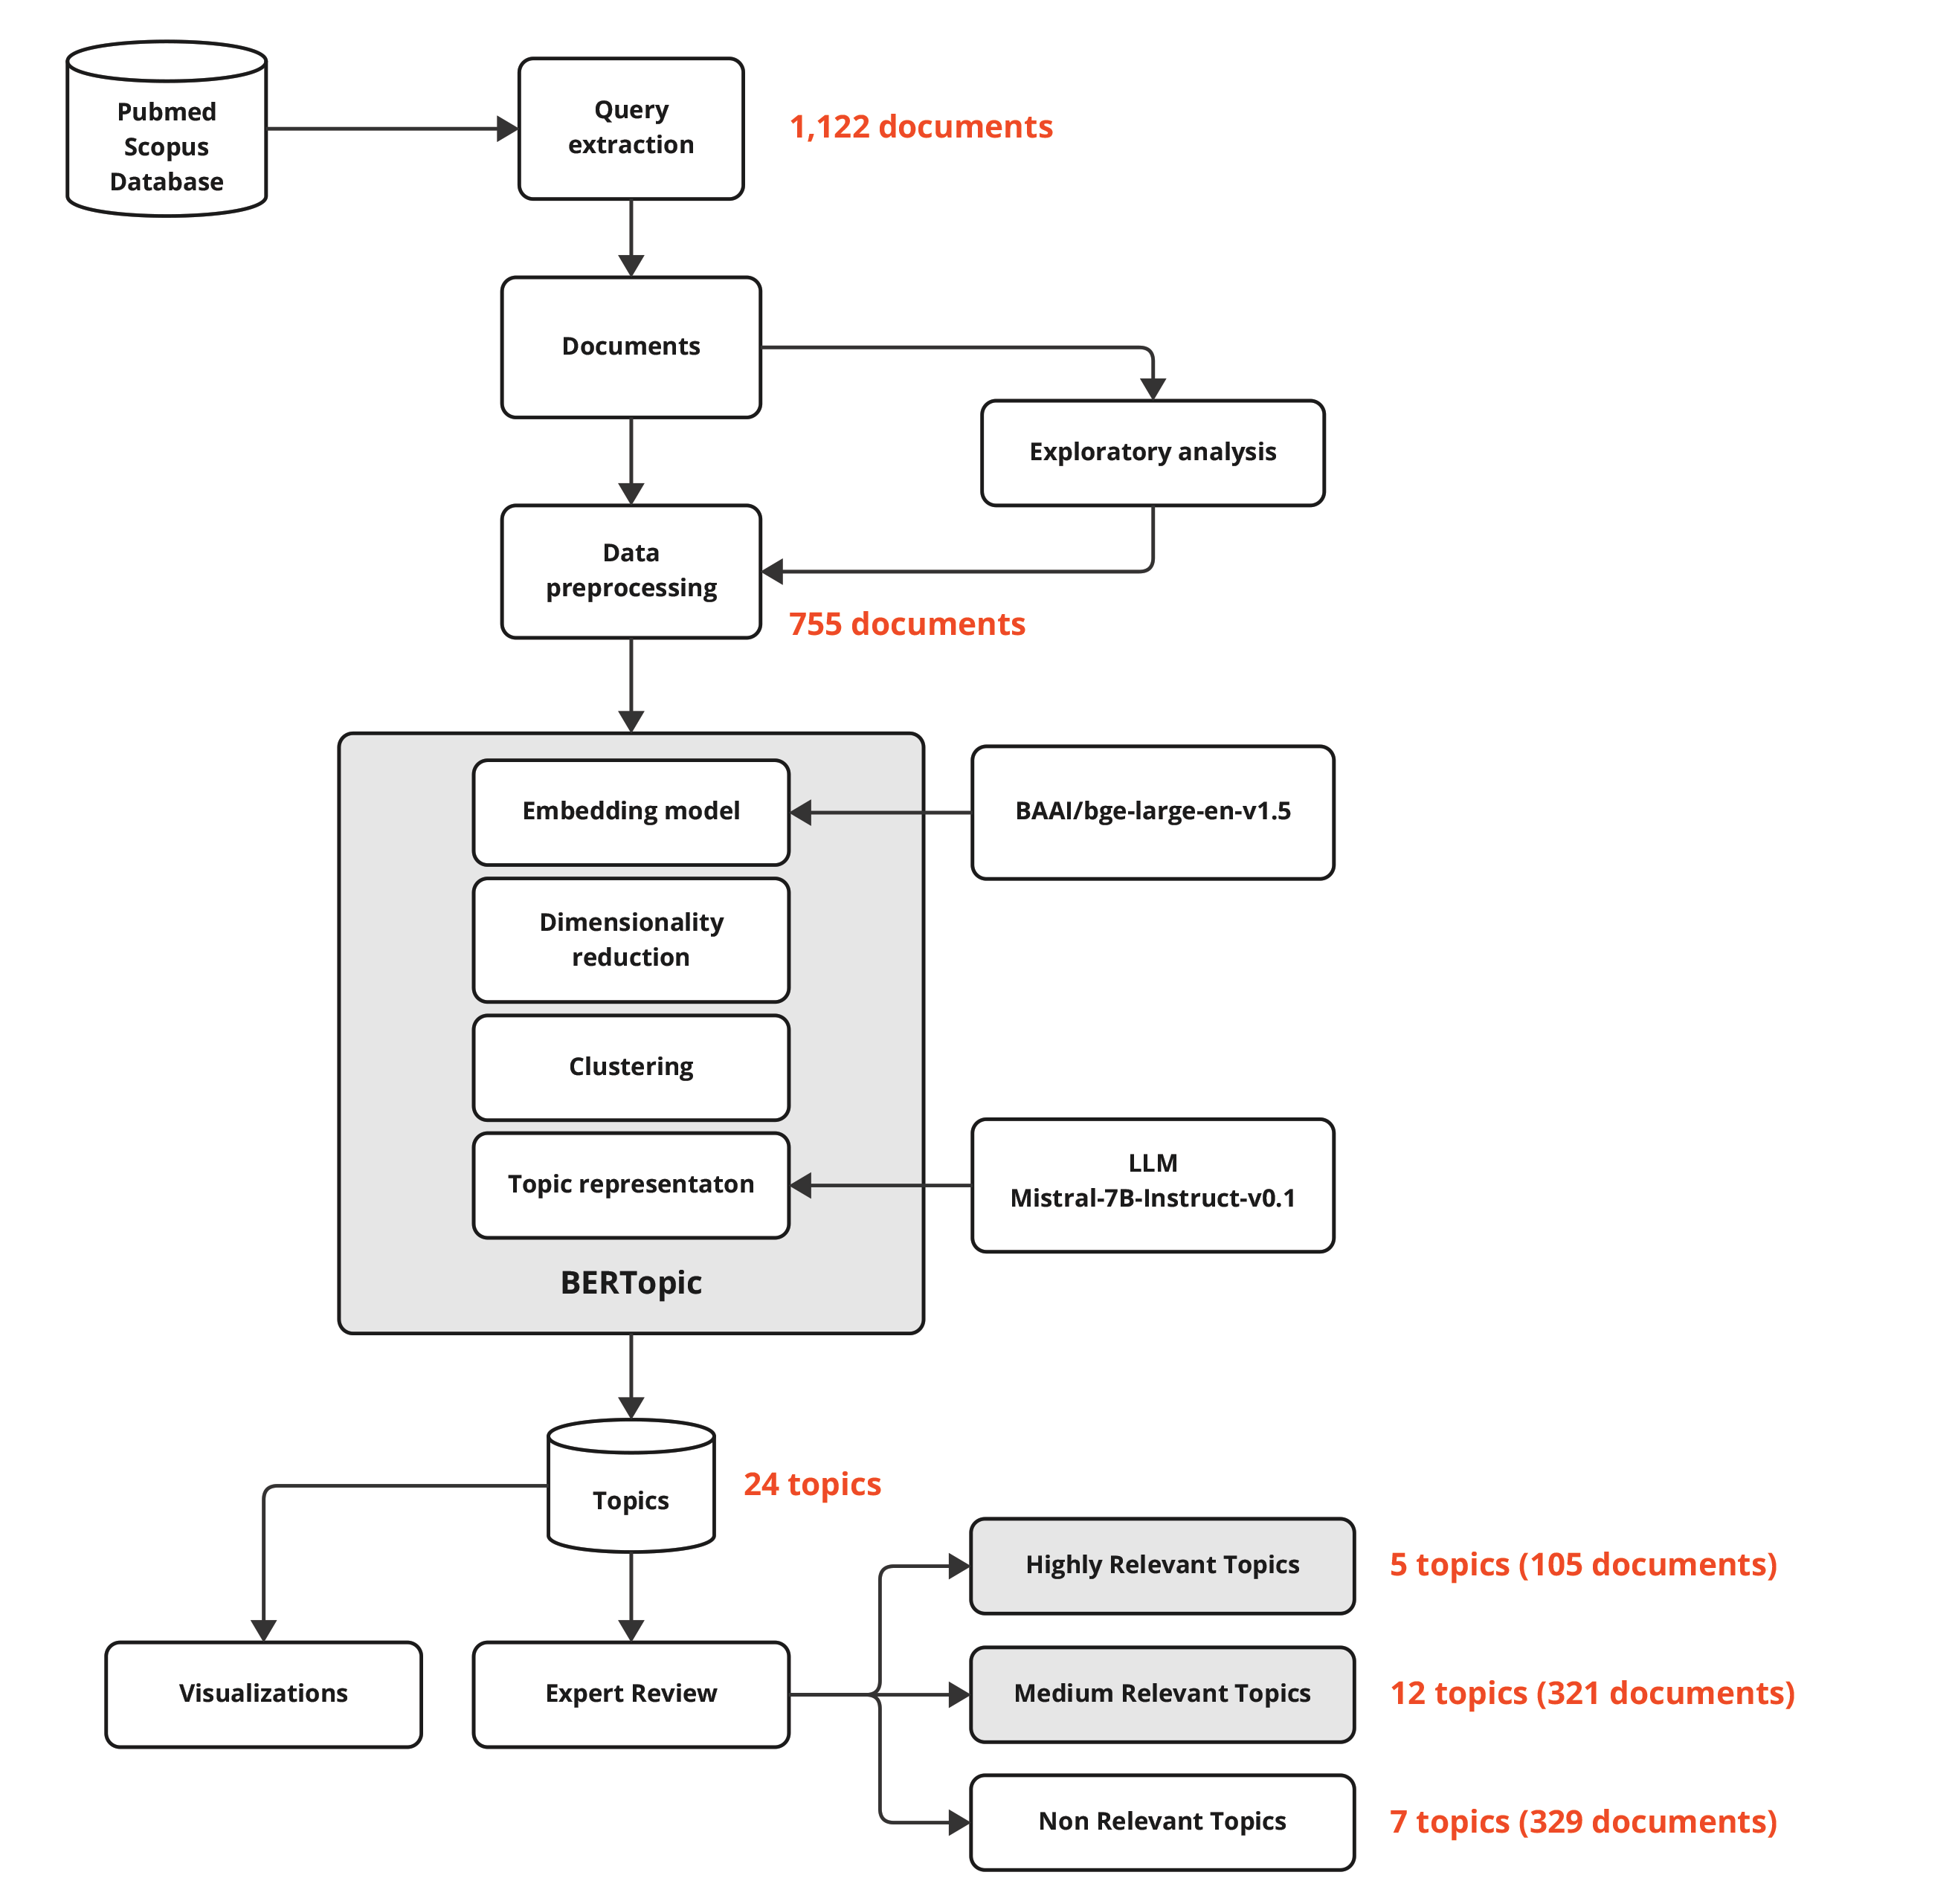
\includegraphics[width=0.8\textwidth]{img/NS-No-Show-SOTA-Workflow.png}
        \caption{\textcolor{blue}{Systematic Topic Review approach for Literature Review process.}}
      \label{fig:STR-workflow}
    \end{figure}




    \begin{table}[ht]
    \centering
    \caption{\textcolor{blue}{Topics and relevance levels in the literature review.}}
    \label{tab:topics_relevance}
    \begin{tabularx}{\textwidth}{@{}lXr@{}}
    \hline
    \textbf{Relevance} & \textbf{Topic} & \textbf{Count} \\ \hline
    High & Predicting and reducing no-shows in healthcare & 38 \\
         & Reducing no-shows through appointment reminders in healthcare & 21 \\
         & Nonattendance at healthcare appointments & 21 \\
         & Patient No-Shows in Healthcare Appointments & 15 \\
         & Predictive modeling for appointment no-shows & 10 \\ \hline
    Medium & Appointment scheduling and overbooking & 109 \\
           & Reducing non-attendance in mental health treatment & 52 \\
           & Screening Programmes and Nonattendance in Women & 25 \\
           & Portal Enrollment and Appointment No-Shows & 24 \\
           & Pediatric Appointment Attendance and Missing Rates & 23 \\
           & Effectiveness of SMS reminders on outpatient appointment attendance & 20 \\
           & Factors associated with non-adherence to follow-up appointments after orthopaedic trauma injuries & 18 \\
           & Effectiveness of SMS reminders for outpatient colonoscopy & 17 \\
           & Postpartum care attendance and predictors & 9 \\
           & Unmet social needs and missed primary care appointments & 9 \\
           & Reducing no-shows in radiology appointments & 8 \\
           & Reducing non-attendance in healthcare through fines & 7 \\ \hline
    \end{tabularx}
    \end{table}


    \subsection*{Operating Room Planning and Scheduling: Reviews and Taxonomies}

    Operating room (OR) planning and scheduling has been one of the most extensively studied topics in healthcare operations management due to its direct impact on hospital efficiency, patient access, resource utilization, and healthcare costs. Operating rooms are among the most resource-intensive hospital units, accounting for a substantial proportion of operational expenditures while serving as a critical bottleneck in surgical care delivery \cite{cardoen2010,barbagallo2015}. Consequently, a large body of literature has emerged to support decision-making processes related to capacity planning, resource allocation, surgery sequencing, and real-time schedule adaptation.
    
    The seminal review by Cardoen et al. \cite{cardoen2010} established one of the most influential frameworks for classifying operating room planning and scheduling problems. Their taxonomy organized the literature according to decision levels, uncertainty representation, performance measures, and optimization methodologies. Since then, several reviews have expanded this framework to incorporate stochastic optimization, simulation-based approaches, machine learning, and artificial intelligence techniques \cite{al-amin2024,bellini2024,chamarthi2025}. Recent systematic reviews indicate that advances in data availability, electronic health records, and computational capabilities have enabled the development of predictive models for surgical duration estimation, operating room utilization forecasting, postoperative resource management, and cancellation prediction \cite{bellini2020,espaillat2024}. These developments reflect the gradual transition from purely deterministic scheduling models toward increasingly data-driven and adaptive decision-support systems.
    
    The literature commonly categorizes operating room planning problems according to their decision scope, resource constraints, objectives, and uncertainty characteristics. Cardoen et al. \cite{cardoen2010} proposed a comprehensive classification that distinguishes between patient-related factors, resource availability, scheduling objectives, and solution methodologies. Other studies have focused on representing surgical processes through standardized workflow models, including Business Process Model and Notation (BPMN), to improve the integration of clinical pathways with quantitative planning tools \cite{barbagallo2015}. More recent taxonomies extend these classifications by incorporating predictive analytics, machine learning, and dynamic scheduling environments capable of adapting to operational disruptions and changing clinical conditions \cite{chamarthi2025}.
    
    A widely accepted paradigm organizes operating room planning decisions into three hierarchical levels. Strategic planning addresses long-term capacity allocation decisions, typically involving the distribution of operating room resources among surgical specialties over annual planning horizons \cite{taylor2023}. Tactical planning focuses on the development of Master Surgical Schedules (MSS), in which operating room blocks are allocated to specialties, departments, or surgical teams on a weekly or monthly basis \cite{jittamai2025,eshghali2024}. Operational planning concerns daily surgery sequencing, staff assignment, and reactive rescheduling activities required to accommodate emergencies, cancellations, and unexpected delays \cite{zhao2025optimizing,eshghali2024,tsang2025}. This hierarchical decomposition remains the dominant framework for structuring operating room optimization problems and provides the conceptual foundation for most contemporary scheduling methodologies.
    
    Despite substantial methodological advances, several challenges remain unresolved. Many optimization models continue to be evaluated using retrospective datasets or simulated environments, limiting evidence regarding their effectiveness in real-world hospital settings \cite{chamarthi2025,bellini2020}. The absence of standardized performance metrics complicates the comparison of optimization strategies and reduces reproducibility across studies \cite{schouten2023}. Furthermore, uncertainty associated with surgical durations, emergency arrivals, cancellations, and downstream resource availability remains insufficiently integrated into strategic and tactical planning models \cite{cardoen2010,al-amin2024}. Finally, although industrial scheduling methodologies have significantly influenced healthcare operations research, relatively few studies have investigated the application of Job Shop Scheduling and Flexible Job Shop Scheduling paradigms using large-scale, real-world datasets from public hospitals. This gap is particularly relevant in resource-constrained healthcare systems, where improving throughput, reducing waiting times, and increasing operating room utilization remain critical operational objectives.

    \subsection*{Exact Optimization Methods for Operating Room Scheduling}

    Exact optimization methods constitute one of the foundational research streams in operating room scheduling, as they provide mathematically rigorous solutions and, under appropriate assumptions, guarantee global optimality. These approaches have been extensively applied to support decision-making processes involving surgery sequencing, operating room allocation, staff assignment, and capacity planning under multiple operational constraints \cite{cardoen2010_review,al-amin2024}. Their relevance is particularly evident in healthcare environments where resource utilization, patient waiting times, overtime costs, and service quality must be simultaneously balanced.
    
    Among exact approaches, Mixed Integer Linear Programming (MILP) has emerged as the most widely adopted methodology. MILP formulations have been successfully employed to address multi-objective surgical scheduling problems, integrating competing objectives such as patient waiting times, operating room utilization, recovery room occupancy, and staff workload balancing \cite{cardoen2010_seq,jittamai2025}. Recent studies have extended these formulations to collaborative healthcare networks, where multiple hospitals coordinate operating room resources to improve regional surgical capacity and reduce system-wide inefficiencies \cite{roshanaei2017}. Furthermore, advanced MILP-based frameworks have incorporated uncertainty through risk-aware formulations, including upper partial moment models and decision-tree structures, allowing planners to explicitly account for variability in surgical durations and resource consumption \cite{maleki2023}.
    
    Because uncertainty is inherent to surgical systems, stochastic programming has become another major research direction. These models explicitly represent uncertain parameters, such as procedure durations, emergency arrivals, and postoperative resource requirements, through probability distributions or scenario-based representations \cite{lamiri2008,denton2011}. Two-stage stochastic formulations are particularly common, where first-stage decisions determine surgery assignments and resource allocations, while second-stage recourse actions account for overtime, idle time, and schedule disruptions \cite{denton2011,lalmazloumian2023}. More recently, stochastic optimization has been integrated with surgeon preference modeling and collaborative surgery planning, enabling the simultaneous consideration of operational performance and clinician satisfaction under uncertainty \cite{azab2024}.
    
    A complementary line of research focuses on robust optimization. Unlike stochastic approaches, robust optimization does not require complete knowledge of probability distributions and instead seeks solutions that remain feasible across predefined uncertainty sets. This characteristic makes robust methods particularly attractive in healthcare environments where reliable probabilistic information may be unavailable or difficult to estimate. Applications include operating room planning during highly uncertain conditions such as the COVID-19 pandemic, where robust optimization models were used to coordinate specialty teams, emergency admissions, and surgical resource allocation under rapidly changing demand patterns \cite{arabmomeni2022}. More recently, distributionally robust optimization frameworks have been proposed to jointly schedule operating rooms and anesthesiologists while mitigating the risk of excessive overtime and schedule instability \cite{tsang2025,fallahpour2024}.
    
    As operating room scheduling problems grow in scale and complexity, decomposition-based exact approaches have become increasingly important. Column generation techniques have been successfully employed to solve large-scale scheduling instances that would otherwise be computationally intractable using monolithic optimization models \cite{lamiri2008}. Recent developments have integrated column generation within hierarchical optimization frameworks that decompose planning decisions across strategic, tactical, and operational levels \cite{zhao2025optimizing}. Some studies have further enhanced these approaches through machine learning and reinforcement learning mechanisms that guide the generation of promising scheduling patterns, thereby accelerating convergence while preserving the mathematical rigor of exact optimization \cite{zhao2025optimizing}.
    
    Despite their strong theoretical foundations and ability to produce optimal or near-optimal solutions, exact optimization methods often face computational challenges when applied to large-scale operating room environments characterized by multiple resources, uncertainty, and dynamic disruptions. As problem size and realism increase, solution times can become prohibitive, motivating the development of metaheuristic and hybrid approaches capable of generating high-quality solutions within practical computational limits. These approaches are discussed in the following section.

    \subsection*{Metaheuristic and Hybrid Approaches for Operating Room Optimization}

    The computational complexity of operating room scheduling problems has motivated the widespread adoption of metaheuristic and hybrid optimization approaches. While exact methods provide mathematically optimal solutions, their applicability is often limited when addressing large-scale environments characterized by multiple resources, stochastic surgical durations, emergency arrivals, and complex operational constraints. Consequently, metaheuristic approaches have become a dominant research direction due to their ability to generate high-quality solutions within practical computational times \cite{cardoen2010_review,al-amin2024,vieira2025}.
    
    Early applications focused on classical metaheuristics such as Genetic Algorithms, Tabu Search, Simulated Annealing, and Variable Neighborhood Search (VNS), which demonstrated strong performance in multi-objective operating room scheduling problems involving patient waiting times, operating room utilization, overtime reduction, and resource balancing \cite{cardoen2010_review,cardoen2010_seq}. These methods are particularly attractive because they can efficiently explore large combinatorial search spaces while accommodating operational constraints that are difficult to model using exact optimization techniques. As healthcare systems have become increasingly complex, metaheuristics have evolved from isolated search procedures toward more sophisticated frameworks capable of integrating multiple decision layers and resource dependencies.
    
    Recent developments have introduced population-based optimization approaches specifically designed for integrated operating room scheduling. Among them, Random-Key Optimizer (RKO) frameworks have attracted considerable attention by representing scheduling decisions through continuous random-key encodings that can be effectively explored by evolutionary search mechanisms \cite{vieira2025}. These approaches facilitate the simultaneous optimization of operating room allocation, surgery sequencing, and resource assignment while maintaining considerable flexibility when adapting to different hospital environments.
    
    A major trend in recent literature is the integration of optimization algorithms with machine learning and artificial intelligence techniques. Reinforcement Learning (RL) has emerged as a promising mechanism for guiding optimization procedures, particularly in large-scale scheduling problems where traditional search strategies become computationally expensive. Recent studies have demonstrated that RL agents can learn scheduling policies capable of identifying promising operating room allocation patterns and supporting decomposition-based exact algorithms such as column generation \cite{zhao2025}. By combining learning and optimization, these hybrid approaches improve solution quality while reducing computational effort.
    
    Another important research direction involves simulation-optimization frameworks. These approaches integrate discrete-event simulation models with optimization algorithms to evaluate scheduling decisions under realistic operating conditions before implementation. Simulation allows researchers to capture stochastic phenomena such as emergency arrivals, surgical duration variability, and downstream resource congestion, while optimization techniques search for schedules that maximize operational performance \cite{xiao2022,frichi2025}. This combination has proven particularly valuable in healthcare environments where uncertainty plays a central role and analytical formulations may oversimplify real-world dynamics.
    
    More recently, the emergence of predict-then-optimize frameworks has strengthened the connection between predictive analytics and operational decision-making. In these approaches, machine learning models are first used to estimate key parameters such as surgical duration, cancellation risk, or patient flow characteristics, and the resulting predictions are subsequently incorporated into optimization models \cite{fairley2019,abbou2022,lex2025}. By improving the quality of input information, these methods can significantly reduce scheduling inefficiencies, increase operating room utilization, and decrease overtime costs.
    
    Although metaheuristic and hybrid approaches generally sacrifice guarantees of global optimality, they offer a favorable trade-off between solution quality and computational efficiency. Their flexibility makes them particularly suitable for large-scale operating room environments characterized by uncertainty, multiple stakeholders, and dynamic operational conditions. Moreover, the growing integration of machine learning, simulation, and optimization techniques suggests that future research will increasingly focus on adaptive decision-support systems capable of continuously learning from hospital operations and responding to changing clinical demands. These developments provide a natural bridge toward industrial scheduling paradigms, particularly Job Shop Scheduling and Flexible Job Shop Scheduling models, which have recently gained attention as promising frameworks for representing surgical systems and optimizing operating room utilization.
    
    \subsection*{Job Shop Scheduling Applications in Healthcare and Operating Rooms}

    The application of industrial scheduling paradigms to healthcare operations has gained increasing attention as hospitals seek to improve resource utilization, patient flow, and operational efficiency. Among these paradigms, Job Shop Scheduling (JSS) and Flexible Job Shop Scheduling (FJSS) provide a natural framework for modeling the complex interactions between surgical procedures, operating rooms, healthcare professionals, and supporting resources. Although many operating room scheduling studies do not explicitly formulate the problem as a job shop scheduling problem, the underlying structure exhibits strong similarities with classical production systems \cite{cardoen2010_review,barbagallo2015}.
    
    From a scheduling perspective, surgical procedures can be interpreted as jobs that require a sequence of interdependent activities, including patient preparation, anesthesia induction, surgery, postoperative cleaning, and recovery processes. Operating rooms act as processing stations where these activities are executed, while surgeons, anesthesiologists, nurses, and specialized equipment constitute additional resources that must be simultaneously available to perform each operation \cite{barbagallo2015,chamarthi2025}. This representation closely resembles resource-constrained scheduling environments commonly studied in manufacturing and project management.
    
    The analogy becomes even stronger when considering Flexible Job Shop Scheduling formulations. In many hospitals, a surgical procedure may be performed in multiple operating rooms with different equipment configurations, staffing arrangements, or specialty capabilities. This flexibility allows scheduling decisions to balance workload across rooms while satisfying clinical and operational constraints \cite{vieira2025}. As a result, FJSS models provide a useful abstraction for capturing the heterogeneous nature of modern surgical systems and the multiple routing alternatives available during schedule construction.
    
    Unlike traditional manufacturing environments, however, healthcare scheduling problems involve additional layers of complexity. Operating room schedules must simultaneously consider the availability of human resources, including surgeons, anesthesiologists, and nursing teams, as well as physical resources such as specialized equipment and operating room capacity. These characteristics naturally lead to Dual Resource Constrained Scheduling formulations, where both human and physical resources must be coordinated throughout the execution of each surgical procedure \cite{roshanaei2017,tsang2025}. Such constraints significantly increase problem complexity while highlighting the need for integrated scheduling approaches.
    
    Another distinguishing feature of healthcare systems is the presence of downstream resource dependencies. The completion of a surgical procedure does not necessarily imply the completion of the patient's treatment pathway, as postoperative recovery units, intensive care beds, and ward capacity often become additional constraints that directly influence operating room utilization. Several studies have therefore proposed integrated scheduling frameworks that extend beyond the operating room itself and explicitly consider downstream resources to prevent bottlenecks that may reduce surgical throughput and increase patient waiting times \cite{fallahpour2024,fairley2019}. This broader perspective aligns closely with production system concepts in which the performance of individual workstations depends on the behavior of the entire process flow.
    
    Recent research has further expanded these concepts by integrating project planning theory, machine learning, and intelligent optimization algorithms into operating room management frameworks \cite{chamarthi2025,zhao2025}. These developments support increasingly adaptive scheduling systems capable of responding to uncertainty, learning from historical data, and dynamically reallocating resources as operational conditions change. Nevertheless, despite the conceptual similarities between operating room scheduling and Job Shop Scheduling, relatively few studies have explored the direct application of JSS and FJSS methodologies using large-scale operational datasets from public hospitals.
    
    This gap is particularly relevant because public healthcare systems often operate under severe resource constraints, high demand variability, and growing surgical waiting lists. Consequently, the adaptation of Job Shop Scheduling methodologies to operating room management represents a promising research direction capable of combining the extensive theoretical foundations of industrial scheduling with the practical challenges of healthcare operations. The present study contributes to this emerging line of research by investigating the applicability of Job Shop Scheduling concepts to the optimization of operating room utilization using multi-year operational data from a public hospital environment.
    
    \subsection*{Performance Metrics for Operating Room Optimization}

    The evaluation of operating room (OR) optimization initiatives remains challenging due to the lack of a universally accepted performance metric. Recent evidence indicates that the most robust assessments rely on multidimensional sets of indicators that jointly measure operational efficiency, service quality, and resource utilization \cite{Schouten2023,Charlesworth2020}. Among the most frequently reported metrics are OR utilization, first-case start-time accuracy, surgical duration estimation accuracy, turnover time, cancellation rates, after-hours surgery rates, and operational costs \cite{Fixler2013,Reeves2020,Negash2022,Sibhatu2024}. Recent studies further advocate the use of composite indicators, such as Operating Room Effectiveness (ORE) and Overall Operating Room Effectiveness (OORE), which integrate planning, performance, and quality losses into a single performance measure \cite{Souza2020,Sonmez2020}. Several authors also caution that optimizing a single metric may negatively affect other critical dimensions of OR performance, recommending instead a systems-oriented evaluation framework that simultaneously considers efficiency, quality of care, patient-centered outcomes, and staff well-being \cite{Basson2018,Schouten2023}. Consequently, the literature converges on the need for a standardized set of complementary indicators to support the objective evaluation and comparison of operating room scheduling and optimization strategies.
 
   \subsection*{Implementation Challenges and Adoption of Optimization Strategies}
   Despite the growing body of research on operating room scheduling and optimization methods, translating these solutions into routine clinical practice remains a significant challenge. Evidence from implementation science suggests that successful adoption depends not only on the technical quality of an intervention but also on its alignment with organizational workflows, stakeholder needs, and institutional constraints \cite{Lam2021,Roberts2020,Wang2023}. Common barriers include limited staff availability, resistance to change, inadequate information systems, lack of leadership support, and poor integration with existing clinical processes \cite{Nair2024,PetersCorbett2023,Sendak2020}. To overcome these obstacles, the literature recommends a systematic assessment of local barriers using established implementation frameworks such as CFIR, i-PARIHS, and PRISM, followed by the deployment of context-specific, multi-component implementation strategies \cite{Lam2021,Roberts2020,Byhoff2023,Yakovchenko2023}. These strategies typically combine leadership engagement, clinical champions, targeted training, workflow redesign, continuous feedback mechanisms, and active stakeholder participation throughout the implementation process \cite{Tong2024,Teggart2024,Ramirez2024,Hassett2024}. Furthermore, long-term sustainability is enhanced when optimization initiatives demonstrate clear operational benefits, impose minimal additional workload, and become embedded within routine organizational practices and information systems \cite{Nair2024,Varsi2019,Eisner2025}. Consequently, implementation considerations should be treated as a critical component of operating room optimization projects, particularly in public healthcare environments where organizational complexity and resource limitations may hinder the realization of expected operational gains.


\textcolor{red}{
Nuestro paper será novedoso en la medida que:
}

\begin{itemize}

\item \textcolor{red}{
Utilizamos y validamos los resultados sobre varios años de datos operacionales reales provenientes de quince pabellones quirúrgicos de un hospital público. Esto contrasta con una parte importante de la literatura, que basa sus evaluaciones en instancias sintéticas, simulaciones o estudios retrospectivos de alcance limitado.
}

\item \textcolor{red}{
Demostramos que ciertas heurísticas de despacho permiten mejorar sistemáticamente la política de programación actualmente utilizada por el hospital, generando mejoras medibles en indicadores como utilización de pabellones, throughput quirúrgico, lead time, tiempos de espera y horas extraordinarias.
}

\item \textcolor{red}{
Proponemos una nueva familia de heurísticas específicamente diseñadas para el entorno quirúrgico, incorporando variables clínicas y operacionales que normalmente no están presentes en las reglas clásicas desarrolladas para sistemas manufactureros.
}

\item \textcolor{red}{
Demostramos que el sistema quirúrgico puede modelarse adecuadamente como un Flexible Job Shop Scheduling Problem, proporcionando evidencia empírica de que los conceptos provenientes de la planificación de talleres de trabajo son aplicables al contexto hospitalario.
}

\item \textcolor{red}{
Mostramos que las reglas de despacho desarrolladas originalmente para entornos industriales pueden transferirse al ámbito quirúrgico y utilizarse como mecanismos efectivos de apoyo a la toma de decisiones operacionales.
}

\item \textcolor{red}{
Cuantificamos el desempeño relativo de distintas reglas de despacho, demostrando que algunas políticas de programación son consistentemente superiores a otras bajo condiciones reales de operación hospitalaria.
}

\item \textcolor{red}{
Contribuimos a reducir la brecha existente entre la investigación en Job Shop Scheduling y la gestión de pabellones quirúrgicos, proporcionando un marco metodológico replicable para otros hospitales públicos con restricciones similares de capacidad y demanda.
}

\end{itemize}
% ================================================================
%***TODO
\section{Methodology and Experimental Design}\label{sec:method}
% ================================================================

This section describes the discrete-event simulation model developed to
evaluate OR dispatching strategies under mixed elective-urgent demand, as
well as the experimental configuration used to compare the six strategies
of interest. The model was implemented in Python using a modular
architecture that allows flexible configuration of policy parameters,
including dispatching rules, assignment modalities, OR dedication, time
windows, and capacity reservation.

% ----------------------------------------------------------------
\subsection{Methodology}
% ----------------------------------------------------------------
The simulation model comprises six interrelated components: surgical
duration modeling, urgent arrival modeling, dispatching rules and
assignment modalities, the central scheduler logic, performance metrics,
and replication design. Each is described below.

\begin{itemize}

  \item \textbf{Surgical Duration Modeling.}
  Surgical durations were parameterized using the total OR time recorded
  in the dataset, grouped by ICD-10 diagnostic code. The 50 most frequent
  ICD-10 codes with at least 30 valid observations are selected. For each
  code, three candidate distributions are fitted via maximum likelihood
  estimation: normal, gamma, and log-normal. Goodness-of-fit is assessed
  using the Kolmogorov-Smirnov (KS) test \cite{strum1997surgical}: if the best
  $p$-value exceeds the significance level $\alpha = 0.05$, the
  distribution yielding the highest $p$-value is selected; otherwise,
  direct empirical sampling from the observed durations for that code is
  used. For codes outside the top 50 or with fewer than 30 observations,
  a gamma distribution fitted globally across all dataset durations is
  applied.

  Let $T_{ij}$ denote the duration of surgery $j$ with diagnosis $i$.
  The model generates durations as:

  \begin{equation}
  T_{ij} \sim \begin{cases}
  F_i(\theta_i) & \text{if } i \in \mathcal{C}_{\text{top}}
  \text{ and KS passed,}\\
  \text{Empirical}(T_{i1}, \ldots, T_{in_i}) & \text{if } i \in
  \mathcal{C}_{\text{top}} \text{ and KS failed,}\\
  \text{Gamma}(\hat{a}, \hat{\text{loc}}, \hat{s}) & \text{if }
  i \notin \mathcal{C}_{\text{top}},
  \end{cases}
  \end{equation}

  where $F_i$ is the selected distribution for code $i$ with parameters
  $\theta_i$, $\mathcal{C}_{\text{top}}$ is the set of frequent codes,
  and $(\hat{a}, \hat{\text{loc}}, \hat{s})$ are the globally fitted
  gamma parameters. A minimum floor of 15 minutes is enforced to prevent
  unrealistic durations. Following each surgery, a turnaround and
  cleaning time is incorporated:

  \begin{equation}
  T_{\text{cleaning}} \sim \text{Uniform}(15, 20) \text{ minutes.}
  \end{equation}

  \item \textbf{Urgent Arrival Modeling.}
  Urgent surgical arrivals are modeled as a non-homogeneous Poisson
  process (NHPP) with rates varying by hour of the day and day of the
  week, capturing the temporal heterogeneity observed in the data \cite{bell2019modeling,alexopoulos2008modeling}. Two complementary estimation approaches were
  implemented.

  Under the \textit{frequentist approach}, for each combination of
  weekday $wd \in \{0, \ldots, 6\}$ and hour $h \in \{0, \ldots, 23\}$,
  the rate is estimated as:

  \begin{equation}
  \hat{\lambda}_{wd}(h) = \frac{n_{wd,h}}{D_{wd}},
  \end{equation}

  where $n_{wd,h}$ is the total number of urgent arrivals observed in
  cell $(wd, h)$ and $D_{wd}$ is the number of days of type $wd$ in the
  dataset. Under the \textit{Bayesian approach via Metropolis-Hastings},
  a smoothed estimate with uncertainty quantification is obtained by
  placing a normal prior on the log-rates:

  \begin{equation}
  \log \lambda_b \sim \mathcal{N}(\mu_0, \sigma_0^2),
  \quad b = 1, \ldots, B,
  \end{equation}

  with $\mu_0 = \log(0.03)$ and $\sigma_0 = 1.0$. The likelihood is
  modeled as Poisson counts per time slot:

  \begin{equation}
  n_b \mid \lambda_b \sim \text{Poisson}(\lambda_b \cdot \Delta_b),
  \end{equation}

  where $\Delta_b$ is the duration of slot $b$ in minutes. Inference is
  performed via Metropolis-Hastings with 5{,}000 iterations, 1{,}500
  burn-in samples, and thinning every 5 iterations \cite{edition2013bayesian}. Within the simulator, the effective intensity per
  time slot is:

  \begin{equation}
  \lambda_{\text{slot}}(wd,h) = \hat{\lambda}_{wd}(h) \cdot \alpha
  \cdot \frac{ts}{60},
  \end{equation}

  where $\alpha$ is a scaling factor calibrated to approximate observed
  urgent arrival volumes. Arrivals per
  slot are then sampled as:

% (see Subsection~\ref{sec:exp})

  \begin{equation}
  N_{\text{slot}} \sim
  \text{Poisson}\left(\lambda_{\text{slot}}(wd,h)\right).
  \end{equation}

  Each urgent case is inserted into the waiting queue only when its
  arrival instant is reached by the simulation clock, preserving
  temporal causality.

  \item \textbf{Dispatching Rules and Assignment Modalities.}
  Three dispatching rules are evaluated for the elective patient queue.
  \textit{FIFO} (First-In, First-Out) orders patients by queue entry
  date from oldest to most recent. \textit{SPT} (Shortest Processing
  Time) orders patients by estimated duration from shortest to longest,
  where the estimate is obtained by sampling from the fitted ICD-10
  distribution at simulation start. \textit{LPT} (Longest Processing
  Time) orders patients by estimated duration from longest to shortest.
  These rules are combined with two OR assignment modalities.
  \textit{Sequential} assignment fills available ORs in order, assigning
  the next patient in queue to the first available OR.
  \textit{Alternating} assignment rotates between care types
  (elective/urgent) per OR, but only when no urgent cases are pending;
  when urgent demand exists, it receives absolute priority. The
  combination of three rules with two modalities yields six evaluated
  strategies. Across all strategies, urgent surgeries take precedence
  over elective cases whenever pending urgent demand exists.

  \item \textbf{Simulation Scheduler Logic.}
  The simulator operates through a centralized scheduler that iterates
  over each simulated day using a discrete clock advancing minute by
  minute. The system is non-preemptive: a surgery once started is never
  interrupted. Cases that cannot begin within a given day remain in the
  queue for the following day. The simulator initializes with empty
  queues (cold start), which may underestimate steady-state congestion
  on the first simulated day; this limitation is discussed in
  Section~\ref{sec:discussion}. Algorithm~\ref{alg:scheduler} presents
  the high-level scheduler logic.

  \begin{algorithm}[H]
  \caption{Central Scheduler (high-level view)}
  \label{alg:scheduler}
  \begin{algorithmic}[1]
  \State Initialize schedule $Q[m,d,s] \gets \emptyset$ and
  $next\_free[q] \gets 0$
  \State Generate urgent event list $E$ with arrival times (NHPP)
  \State Sort elective queue according to selected rule (FIFO/SPT/LPT)
  \For{$day \gets 1$ \textbf{to} $d$}
    \State $t \gets 0$
    \While{$t < s$}
      \State Release into urgent queue all cases with arrival $\leq$
      current time
      \State $OR\_free \gets \{q : next\_free[q] \leq t\}$
      \If{$OR\_free$ is empty}
        \State $t \gets \min_q next\_free[q]$
        \State \textbf{continue}
      \EndIf
      \For{\textbf{each} $q$ \textbf{in} $OR\_free$}
        \State Determine eligibility based on time window and
        exclusivity/reservation policy
        \State Select care type: urgent if pending urgent demand
        exists; elective otherwise
        \State Attempt to assign surgery $+$ cleaning in
        $Q[q, day, \cdot]$ from $t$
        \If{assignment fits in schedule}
          \State Update $next\_free[q]$, metrics, and queues
        \EndIf
      \EndFor
      \State Advance $t$ to next relevant event
    \EndWhile
  \EndFor
  \end{algorithmic}
  \end{algorithm}

  \item \textbf{Performance Metrics.}
  Three primary metrics are reported. \textit{Throughput} is the total
  number of surgeries completed over the simulated horizon:

  \begin{equation}
  \text{Throughput} = \#\{\text{completed surgeries}\}.
  \end{equation}

  \textit{Utilization} is the percentage of time slots occupied by
  active surgery relative to total available slots:

  \begin{equation}
  \text{Utilization}~(\%) = 100 \cdot
  \frac{\text{surgery-occupied slots}}{m \cdot d \cdot s}.
  \end{equation}

  \textit{Lead time} is the average time from the start of the simulated
  horizon to the completion of each surgery, expressed in days:

  \begin{equation}
  \text{Lead time}~(\text{days}) = \frac{1}{\text{Throughput}}
  \sum_{i=1}^{\text{Throughput}}
  \frac{t_i^{\text{end}} - t_0}{24 \cdot 3600},
  \end{equation}

  where $t_0$ is the horizon start and $t_i^{\text{end}}$ is the
  completion time of surgery $i$. Lead time as defined here measures
  the average temporal position at which surgeries are completed within
  the horizon, not the individual waiting time from queue entry; a
  lower lead time indicates production concentrated in earlier phases
  of the horizon.

  \item \textbf{Replication Design and Statistical Analysis.}
  Each strategy is evaluated over $R = 30$ independent replications,
  each using a distinct pseudo-random seed. For each metric $Y$, the
  sample mean $\bar{Y}$ and a 95\% confidence interval based on the
  Student's $t$-distribution are reported:

  \begin{equation}
  \text{CI}_{95\%} = \bar{Y} \pm t_{R-1,\, 0.025} \cdot
  \frac{s_Y}{\sqrt{R}},
  \end{equation}

  where $s_Y$ is the sample standard deviation across the $R$
  replications.

\end{itemize}

% ----------------------------------------------------------------
\subsection{Experimental Design}
% ----------------------------------------------------------------

Six strategies are compared, resulting from combining three dispatching
rules (FIFO, SPT, and LPT) with two assignment modalities (sequential
and alternating). The experimental setup is structured around the
following components.


\begin{itemize}

  \item \textbf{Base configuration.}
  The base case uses ten ORs operating 24 hours over five consecutive
  days, with a temporal resolution of one minute. The first 500 patients
  in the elective queue, ordered by system entry date, are processed.
  Tables~\ref{tab:params_sim}, \ref{tab:params_policy}, and
  \ref{tab:strategies} summarize the global simulation parameters,
  policy parameters, and evaluated strategies, respectively.

  \begin{table}[ht]
  \centering
  \caption{Global simulation parameters (base case).}
  \label{tab:params_sim}
  \begin{tabular}{ll}
  \toprule
  Parameter & Value \\
  \midrule
  Elective patients ($N$) & 500 \\
  Operating rooms ($m$) & 10 \\
  Horizon ($d$ days) & 5 \\
  Hours per day & 24 \\
  Temporal resolution ($ts$) & 1 minute \\
  Horizon start ($t_0$) & 2025-10-06 00:00:00 \\
  Independent replications ($R$) & 30 \\
  Random seeds & $\{1, 2, \ldots, 30\}$ \\
  \bottomrule
  \end{tabular}
  \end{table}

  \begin{table}[ht]
  \centering
  \caption{Policy parameters used in the base run.}
  \label{tab:params_policy}
  \begin{tabular}{ll}
  \toprule
  Parameter & Value \\
  \midrule
  Urgent arrival scaling factor ($\alpha$) & 0.1 \\
  Cleaning time & Uniform(15, 20) min \\
  Elective capacity reservation & 0\% \\
  Exclusive ORs (urgent) & 0 \\
  Exclusive ORs (elective) & 0 \\
  Exclusivity mode & Mixed \\
  Urgent time window & 00:00 -- 24:00 (unrestricted) \\
  Elective time window & 00:00 -- 24:00 (unrestricted) \\
  \bottomrule
  \end{tabular}
  \end{table}

  \begin{table}[ht]
  \centering
  \caption{Evaluated strategies.}
  \label{tab:strategies}
  \begin{tabular}{ll}
  \toprule
  Strategy & Configuration \\
  \midrule
  SPT + Sequential  & SPT rule, sequential assignment \\
  FIFO + Sequential & FIFO rule, sequential assignment \\
  LPT + Sequential  & LPT rule, sequential assignment \\
  SPT + Alternating & SPT rule, alternating assignment \\
  FIFO + Alternating & FIFO rule, alternating assignment \\
  LPT + Alternating & LPT rule, alternating assignment \\
  \bottomrule
  \end{tabular}
  \end{table}

  \item \textbf{Parameter justification.}
  The selection of 10 ORs reflects the current simulator configuration;
  confirmation of the exact number of simultaneously active theaters
  will be incorporated following operational validation with hospital
  staff. The 5-day horizon represents a standard operating week. The
  24/7 schedule reflects the continuous nature of urgent surgical
  demand, although in practice elective activity is concentrated in
  daytime hours, an aspect to be evaluated in future experiments with
  differentiated time windows.

  \item \textbf{Urgent arrival calibration.}
  The scaling factor $\alpha = 0.1$ was selected through manual
  calibration to approximate observed urgent arrival volumes in the
  hospital records. Direct NHPP estimation with $\alpha = 1.0$
  overestimates real arrivals, likely because the model does not capture
  institutional filters regulating actual urgent case flow to the OR.

  \item \textbf{Cold start and warm-up.}
  The cold-start initialization implies that the first simulated day may
  not represent steady-state conditions. Given the 5-day horizon and
  ample installed capacity, this effect is expected to dissipate
  rapidly; however, a formal warm-up period is proposed as a future
  extension.

\end{itemize}


% ================================================================
\section{Data}\label{sec:data}
% ================================================================

This section describes the clinical-operational dataset used to
parameterize the simulation model, including its origin, scope,
preprocessing pipeline, and descriptive characterization. All records
were obtained from the hospital information system and anonymized at
source prior to analysis.

% ----------------------------------------------------------------
\subsection{Data source}\label{data}
% ----------------------------------------------------------------

The data used in this study originate from clinical-operational records
of Hospital Puerto Montt Dr.\ Eduardo Schütz Schroeder, a
high-complexity referral facility belonging to the Servicio de Salud
del Reloncaví, located in the Los Lagos Region, Chile. The hospital
operates 12 surgical theaters (\textcolor{red}{identified as Q-2 through Q-15}) and
serves an annual volume of approximately 7{,}000 surgical interventions
across 21 specialties.

The dataset comprises 28{,}464 intervention records spanning from
January 2, 2020 to December 30, 2023. Each record includes an
anonymized patient identifier, date and time of OR entry and
intervention, postoperative diagnosis coded in ICD-10, care type
(scheduled, urgent, or unscheduled), surgical specialty, intervention
and anesthesia times, procedures performed, and surgical team
composition. Table~\ref{tab:dataset_summary} summarizes the main
characteristics of the dataset.

\begin{table}[]
\centering
\caption{Descriptive summary of the Hospital Puerto Montt dataset
(2020--2023).}
\label{tab:dataset_summary}
\begin{tabular}{ll}
\toprule
Characteristic & Value \\
\midrule
Total records & 28{,}464 \\
Study period & January 2020 -- December 2023 \\
Surgical theaters & 12 \\
Surgical specialties & 21 \\
Unique ICD-10 codes & 1{,}589 \\
\midrule
\multicolumn{2}{l}{\textbf{Distribution by care type}} \\
\quad Scheduled & 27{,}042 (95.0\%) \\
\quad Urgent & 1{,}278 (4.5\%) \\
\quad Unscheduled & 143 (0.5\%) \\
\quad No record & 1 ($<$0.01\%) \\
\midrule
\multicolumn{2}{l}{\textbf{Total OR time (minutes)}} \\
\quad Mean $\pm$ SD & $134.7 \pm 97.9$ \\
\quad Median (IQR) & 112.0 (71.0 -- 168.0) \\
\bottomrule
\end{tabular}
\end{table}

% ----------------------------------------------------------------
\subsection{Cleaning and pre-processing}\label{Data-cleaning}
% ----------------------------------------------------------------

The preprocessing pipeline comprised the following stages. First,
records with missing or inconsistent temporal fields were removed,
including cases where the recorded end time preceded the start time.
Second, all date and time fields were converted to a standardized
format, and derived time variables were computed, including
intervention duration, total OR time, and transition times between
successive perioperative stages (OR entry, anesthetic induction,
intervention start and end, OR exit, and recovery entry and exit).
Third, ICD-10 code consistency was verified, preserving the hospital's
original coding scheme; codes with fewer than 30 observations were
grouped under a generic category for the purposes of distribution
fitting, as described in Section~\ref{sec:method}.

It is important to note that the 2020--2023 study period encompasses
the operational impact of the COVID-19 pandemic on surgical activity,
including phases of elective surgery suspension and OR reconfiguration. These periods were not excluded from the dataset,
as they reflect the actual operational conditions of the hospital.
However, this aspect should be considered when interpreting the
estimated duration distributions and urgent arrival rates, as pandemic
disruptions may have altered the underlying demand patterns relative
to a pre-pandemic baseline.

% ----------------------------------------------------------------
\subsection{Descriptive analysis}\label{descriptive-statistics}
% ----------------------------------------------------------------

This subsection characterizes the two demand streams modeled in the
simulation: urgent surgical arrivals and the elective caseload,
the latter described through its ICD-10 composition.

\subsection*{Urgent demand characterization}

Of the 28{,}464 total records, 1{,}421 correspond to surgeries
classified as urgent or unscheduled, representing 4.99\% of the total
surgical volume. Analysis of the temporal distribution of urgent
arrivals reveals significant heterogeneity by hour of the day and day
of the week, motivating the use of a
non-homogeneous Poisson process (NHPP) for arrival modeling rather
than a stationary process. The estimation of NHPP rates is detailed
in Section~\ref{sec:method}. Figure~\ref{fig:urgent_heatmap} presents
the observed urgent arrival rates by weekday and hour, illustrating
the temporal structure captured by the model.

\subsection*{Most frequent diagnoses}

Table~\ref{tab:top_cie10} presents the ten most frequent ICD-10 codes
in the dataset, which together account for a substantial share of the
total surgical volume. The predominance of ophthalmological procedures
(cataracts), orthopedic cases (fractures), and general surgery
(cholelithiasis) is consistent with the profile of a high-complexity
hospital serving both high-frequency elective demand and traumatological
emergencies. This diagnostic composition directly informs the duration
modeling strategy described in Section~\ref{sec:method}, as the most
frequent codes are individually parameterized while less frequent ones
are handled through a global distribution.

\begin{table}[]
\centering
\caption{Ten most frequent ICD-10 codes in the dataset.}
\label{tab:top_cie10}
\begin{tabular}{llr}
\toprule
ICD-10 & Abbreviated description & $n$ \\
\midrule
H25.1 & Nuclear senile cataract         & 1{,}875 \\
H26.9 & Unspecified cataract            & 787 \\
K80.2 & Calculus of gallbladder without cholecystitis & 653 \\
S52.5 & Fracture of lower end of radius & 532 \\
S72.0 & Fracture of neck of femur       & 355 \\
H11.0 & Pterygium                        & 332 \\
S82.6 & Fracture of lateral malleolus   & 330 \\
H25.0 & Incipient senile cataract        & 319 \\
C50.9 & Malignant neoplasm of breast, unspecified & 302 \\
K80.0 & Calculus of gallbladder with acute cholecystitis & 288 \\
\bottomrule
\end{tabular}
\end{table}

% \section{Modeling}\label{Modeling}
    
%     \subsection{Feature selection}\label{Feature-selection}    

%     In sit amet tempor lorem. Curabitur non ultrices magna. Vestibulum rhoncus quis sapien a ultricies. In vitae nibh quam. Curabitur laoreet lacus at justo dignissim, a faucibus orci molestie. 


    

%     In sit amet tempor lorem. Curabitur non ultrices magna. Vestibulum rhoncus quis sapien a ultricies. In vitae nibh quam. Curabitur laoreet lacus at justo dignissim, a faucibus orci molestie. 
    
%     \begin{align}
%         V = \sum{\frac{\chi^2 / N}{\min(k-1, r-1)}}\label{V}
%     \end{align}
    


        

    
%         \begin{figure}[!ht]
%             \centering
%             \includegraphics[width=0.8\textwidth]{img/data_science/Combined_Cramer_V_Heatmaps.png}
%             \caption{Combined Cramér's V Test heatmap; all data (left), and with a mask $> 0.8$ applied (right). We observe a few features with high values (red dots).}
%             \label{fig:Combined_Cramer_V_Heatmaps}
%     \end{figure}
    



%     \subsection{Experiment modeling}\label{Exp_Modeling}
    
%     TIn sit amet tempor lorem. Curabitur non ultrices magna. Vestibulum rhoncus quis sapien a ultricies. In vitae nibh quam. Curabitur laoreet lacus at justo dignissim, a faucibus orci molestie. 

% \begin{table}[ht]
%     \centering
%     \caption{Summary of Experiments}
%     \label{tab:experiments}
%     \begin{tabularx}{\textwidth}{@{}lXc@{}}
%         \hline
%         \textbf{Experiment} & \textbf{Description} & \textbf{Trials} \\ \hline
%         EXP1.1 & Baseline model using Logistic Regression to establish initial metrics. & 1 \\
%         EXP1.2 & Baseline comparison with Support Vector Machine (SVM). & 1 \\
%         EXP2.1 & Logistic Regression Classifier highly parameterized using undersampled data. & 30 \\
%         EXP2.1 & Logistic Regression Classifier highly parameterized using oversampled data. & 30 \\
%         EXP3.1 & Apply XGBoost (Boosting) with undersampled data. & 30 \\
%         EXP3.2 & Apply XGBoost (Boosting) with oversampled data. Noted for superior performance in state-of-the-art studies. & 30 \\
%         EXP4.1 & Random Forest Classifier (Bagging) with undersampled data. Used to manage the dataset complexity and imbalance. & 30 \\
%         EXP4.2 & Random Forest Classifier (Bagging) with oversampled data. This model compares with the state-of-the-art. & 30 \\
%         EXP5.1 & Deep Learning via Multi-Layer Perceptron Classifier to explore complex patterns using undersampled data. & 5 \\
%         EXP5.2 & Deep Learning via Multi-Layer Perceptron Classifier using oversampled data. & 5 \\ \hline
%     \end{tabularx}
% \end{table}




%     \subsection{... algorithm}\label{optimization}
    

%     \begin{algorithm}
%         \caption{Optimization Algorithm for Minimizing the Objective Function}
%         \begin{algorithmic}[1]
%         \State \textbf{Initialize:} Set number of folds, $K$, hyper-parameter search space, $S$, and trials, $T$
%         \State \textbf{Define} Objective Function $OF$
%         \Procedure{OptimizeModel}{}
%             \For{$t = 1$ to $T$ }
%                 \State{Select a set of hyper-parameters in $S$}
%                 \State Initialize cross-validation scores
%                 \For{$i = 1$ to $K$}
%                     \State Train model on fold $i$ with current parameters
%                     \State Compute performance metrics on the validation set
%                     \State Compute $runningScore = 1/(F1\_score + \epsilon)$ 
%                     \State Update cross-validation $runningScore$
%                     \If{performance decreases}
%                         \State \textbf{prune} trial $t$
%                     \EndIf
%                 \EndFor
%                 \State Compute $OF$ based on accumulated metrics and penalty
%                 \If{$OF$ is minimized}
%                     \State Update best parameters
%                 \EndIf 
%             \EndFor
%         \EndProcedure
%         \State \textbf{Output:} Best parameter set that minimizes $OF$
%         \end{algorithmic}
%         \label{alg:optimization_algorithm}
%     \end{algorithm}

%  In sit amet tempor lorem. Curabitur non ultrices magna. Vestibulum rhoncus quis sapien a ultricies. In vitae nibh quam. Curabitur laoreet lacus at justo dignissim, a faucibus orci molestie. 



% ================================================================
\section{Results}\label{sec:results}
% ================================================================

This section presents the comparative performance of the six evaluated
strategies across the three primary metrics: throughput, OR utilization,
and lead time. Results are reported for the base experimental
configuration described in Section~\ref{sec:method}. Confidence
intervals over 30 independent replications are reported alongside
point estimates to characterize result variability across random seeds.

% ----------------------------------------------------------------
\subsection{Experiments}\label{sec:exp}
% ----------------------------------------------------------------

Table~\ref{tab:main_results} summarizes the comparative performance of
the six strategies for the base run. The results show consistent
differentiation across dispatching rules, with smaller differences
attributable to the assignment modality within each rule.

\begin{table}[]
\centering
\caption{Aggregate results by strategy (base run, $\alpha = 0.1$,
reservation = 0\%).}
\label{tab:main_results}
\begin{tabular}{lccc}
\toprule
Strategy & Throughput & Utilization (\%) & Lead time (days) \\
\midrule
SPT + Sequential  & 581 & 79.99 & 1.85 \\
FIFO + Sequential & 519 & 79.22 & 2.47 \\
LPT + Sequential  & 383 & 83.29 & 2.93 \\
SPT + Alternating & 581 & 79.99 & 1.86 \\
FIFO + Alternating & 523 & 79.30 & 2.43 \\
LPT + Alternating & 384 & 83.19 & 2.94 \\
\bottomrule
\end{tabular}
\end{table}

\begin{table}[]
\centering
\caption{Best-performing strategy per metric.}
\label{tab:best_by_metric}
\begin{tabular}{lll}
\toprule
Metric & Best strategy & Value \\
\midrule
Throughput  & SPT + Sequential / SPT + Alternating & 581 \\
Utilization & LPT + Sequential & 83.29\% \\
Lead time   & SPT + Sequential & 1.85 days \\
\bottomrule
\end{tabular}
\end{table}

Table~\ref{tab:ci_results} reports the mean and 95\% confidence
intervals for each metric \textcolor{blue}{across 30 independent replications}.

\begin{table}[]
\centering
\caption{Mean and 95\% confidence intervals over 30 replications
by strategy and metric.}
\label{tab:ci_results}
\begin{tabular}{lccc}
\toprule
Strategy & Throughput & Utilization (\%) & Lead time (days) \\
         & Mean (CI)  & Mean (CI)        & Mean (CI) \\
\midrule
SPT + Sequential   & \textbf{[AQUI 1]} & \textbf{[AQUI 1]} & \textbf{[AQUI 1]} \\
FIFO + Sequential  & \textbf{[AQUI 1]} & \textbf{[AQUI 1]} & \textbf{[AQUI 1]} \\
LPT + Sequential   & \textbf{[AQUI 1]} & \textbf{[AQUI 1]} & \textbf{[AQUI 1]} \\
SPT + Alternating  & \textbf{[AQUI 1]} & \textbf{[AQUI 1]} & \textbf{[AQUI 1]} \\
FIFO + Alternating & \textbf{[AQUI 1]} & \textbf{[AQUI 1]} & \textbf{[AQUI 1]} \\
LPT + Alternating  & \textbf{[AQUI 1]} & \textbf{[AQUI 1]} & \textbf{[AQUI 1]} \\
\bottomrule
\end{tabular}
\end{table}

Figures~\ref{fig:spt_sec}--\ref{fig:lpt_alt} present the Gantt
diagrams for each strategy over the five-day simulated horizon,
providing a visual representation of OR occupation patterns, surgery
block distribution, and urgent case insertion across all ten theaters.

\begin{figure}[]
\centering
\includegraphics[width=\textwidth]{gantt_SPTSecuencial_urgencias.png}
\caption{Gantt diagram for the SPT + Sequential strategy.}
\label{fig:spt_sec}
\end{figure}

\begin{figure}[]
\centering
\includegraphics[width=\textwidth]{gantt_FIFOSecuencial_urgencias.png}
\caption{Gantt diagram for the FIFO + Sequential strategy.}
\label{fig:fifo_sec}
\end{figure}

\begin{figure}[]
\centering
\includegraphics[width=\textwidth]{gantt_LPTSecuencial_urgencias.png}
\caption{Gantt diagram for the LPT + Sequential strategy.}
\label{fig:lpt_sec}
\end{figure}

\begin{figure}[]
\centering
\includegraphics[width=\textwidth]{gantt_SPTAlternado_urgencias.png}
\caption{Gantt diagram for the SPT + Alternating strategy.}
\label{fig:spt_alt}
\end{figure}

\begin{figure}[]
\centering
\includegraphics[width=\textwidth]{gantt_FIFOAlternado_urgencias.png}
\caption{Gantt diagram for the FIFO + Alternating strategy.}
\label{fig:fifo_alt}
\end{figure}

\begin{figure}[]
\centering
\includegraphics[width=\textwidth]{gantt_LPTAlternado_urgencias.png}
\caption{Gantt diagram for the LPT + Alternating strategy.}
\label{fig:lpt_alt}
\end{figure}

\FloatBarrier

% ----------------------------------------------------------------
\subsection{Dispatching Rule and Assignment Modality Analysis}
% ----------------------------------------------------------------

\textbf{Dispatching rule effect.} SPT strategies achieve the highest
throughput (581 surgeries under both modalities) and the lowest lead
time (1.85 and 1.86 days), with utilization near 80\%. This outcome
is consistent with the established theoretical properties of SPT in
single-machine scheduling, where prioritizing shorter jobs minimizes
mean flow time. In the present
context, completing shorter procedures first releases OR capacity more
rapidly, enabling a greater number of surgeries to be initiated within
the fixed five-day horizon. The advantage of SPT is further amplified
by the diagnostic composition of the Hospital Puerto Montt dataset,
where a substantial proportion of procedures are short-duration
interventions such as cataract surgery and minor orthopedic procedures.

FIFO yields intermediate performance, with throughput between 519 and
523 and lead time between 2.43 and 2.47 days. By sequencing cases in
arrival order without discriminating by duration, FIFO produces a
heterogeneous mix of procedure lengths per OR, reducing temporal
packing efficiency relative to SPT while avoiding the systematic
disadvantage imposed on long procedures that characterizes SPT.

LPT achieves the highest utilization (above 83\%) but the lowest
throughput (383--384 surgeries) and the highest lead time (2.93--2.94
days). The elevated utilization reflects the fact that long procedures
occupy extended time blocks with a proportionally smaller contribution
from cleaning intervals, but at the cost of completing fewer total
surgeries within the horizon. This result illustrates a key operational
insight: maximizing OR utilization does not imply maximizing
surgical throughput or minimizing patient lead time, a finding
consistent with the broader OR scheduling literature
\cite{cardoen2010operating,guerriero2011operational,may2011surgical}.

\textbf{Assignment modality effect.} Differences between sequential
and alternating modalities are minor within each dispatching rule.
Under SPT, throughput and utilization are identical across modalities,
with a marginal lead time difference of 0.01 days. Under FIFO,
the alternating modality yields a slight throughput gain (+4 surgeries)
and a marginal lead time reduction (--0.04 days). Under LPT, the
alternating modality produces a minimal throughput increase (+1 surgery)
with a negligible lead time variation. These results indicate that,
under the base configuration, \textbf{the dispatching rule is the
primary determinant of system performance, while the assignment
modality has a secondary and largely negligible effect}.

A plausible explanation is that, at the calibrated urgent arrival
scaling factor of $\alpha = 0.1$, the urgent caseload is relatively
low, leaving limited scope for the alternating modality to produce
differential effects. Under higher urgent demand scenarios, the
assignment modality may acquire greater operational relevance, a
hypothesis to be evaluated in future sensitivity analyses.

\textbf{Visual analysis.} The Gantt diagrams in
Figures~\ref{fig:spt_sec}--\ref{fig:lpt_alt} reinforce the
quantitative interpretation. SPT strategies display rapid OR
turnover with shorter, denser surgery blocks and flexible insertion
of urgent cases throughout the horizon. LPT strategies show
continuous extended blocks with sustained high occupancy but lower
case count. FIFO strategies exhibit an intermediate pattern, with
heterogeneous block lengths reflecting the undiscriminated duration
mix. Differences between sequential and alternating modalities are
visually minor within each dispatching rule, consistent with the
quantitative analysis.

% ----------------------------------------------------------------
\subsection{Discussion}\label{sec:discussion}
% ----------------------------------------------------------------

The findings of this study provide operational evidence for the
comparative performance of simple dispatching rules in a mixed
elective-urgent OR system parameterized with real data from a Chilean
public hospital. The clear dominance of SPT in throughput and lead
time, combined with the secondary role of the assignment modality,
has direct implications for OR management in resource-constrained
public settings: simple, interpretable rules are capable of producing
meaningful performance differences without requiring complex
optimization infrastructure.

The trade-off between utilization and throughput observed under LPT
versus SPT is particularly relevant for decision-makers who may
conflate high OR occupancy with efficient surgical production. The
results demonstrate that these objectives are not equivalent and may
in fact be in tension, reinforcing the need for multi-metric
evaluation frameworks when assessing OR performance \cite{schouten2023}.

Several limitations of the present study should be acknowledged.
First, the cold-start initialization may underestimate steady-state
congestion on the first simulated day; a formal warm-up period is
proposed as a future extension. Second, the urgent
arrival scaling factor $\alpha = 0.1$ was determined through manual
calibration, and a more rigorous calibration procedure tied to
observed case volumes would strengthen the model's fidelity. Third,
the simulation does not currently account for surgeon availability,
anesthesiologist constraints, or specialty-specific OR allocation
policies, all of which represent relevant operational constraints in
practice \cite{tsang2025}. Fourth, the 2020--2023 study period
includes pandemic-related disruptions that may have altered the
underlying demand patterns relative to a stable operational baseline \cite{campos2024examining}.

Future work will extend the current framework along three axes.
First, sensitivity analyses will evaluate the effect of varying
urgent demand levels ($\alpha$), OR dedication policies, and
differentiated time windows on strategy rankings. Second, the
simulation horizon will be extended and a formal warm-up period
will be incorporated to better approximate steady-state behavior.
Third, the framework will serve as a benchmark for evaluating more
sophisticated approaches such as stochastic optimization and
metaheuristic methods, for which the present results provide an
empirically grounded baseline.

% ----------------------------------------------------------------
\subsection{Key Contributions}
% ----------------------------------------------------------------

This study makes three contributions to the operational management
of surgical services in public hospital settings. First, it
provides a minute-by-minute discrete-event simulation model directly
parameterized with real clinical-operational data from a Chilean
public hospital, incorporating empirically derived surgical duration
distributions by ICD-10 code and a Bayesian non-homogeneous Poisson
process for urgent arrival modeling. To the best of our knowledge,
this represents the first simulation study of its kind parameterized
with real data from a Chilean public hospital in the context of
mixed elective-urgent OR scheduling.

Second, it delivers a systematic empirical comparison of six
strategies combining three dispatching rules with two assignment
modalities under a consistent experimental framework, evaluated
over 30 independent replications with 95\% confidence intervals.
The results establish SPT as the dominant rule for throughput and
lead time under the evaluated conditions, while revealing the
limited marginal impact of the assignment modality at low urgent
demand levels.

Third, it establishes an extensible simulation platform that
accommodates additional policy configurations including capacity
reservation, OR dedication, and differentiated time windows,
providing an empirical foundation for future work on more
sophisticated OR planning approaches in resource-constrained
public healthcare systems.


\section{Conclusions}
The implementation of a machine learning-based optimization model to manage the no-show problem in primary In sit amet tempor lorem. Curabitur non ultrices magna. Vestibulum rhoncus quis sapien a ultricies. In vitae nibh quam. Curabitur laoreet lacus at justo dignissim, a faucibus orci molestie. 
 

\backmatter

\bmhead{Acknowledgements}
The authors wish to express their gratitude to Dr. Marusella González, MSc, Head of the Communal Health Directorate, Castro Municipal Corporation, for her generosity in sharing her knowledge and expertise in support of this study.

\bmhead{Author Contribution} 
Authors A.L-A. and C.C.: Conceptualization, problem modeling, methodology, software, writing, and revising. Authors H.K. and Z.P.: Supervision and revision. All authors provided critical feedback and helped the manuscript. All authors have read and approved the manuscript. 

\bmhead{Fundings}
The authors did not receive support from any organization for the submitted work.


\section*{Declarations}

\bmhead{Ethical Approval} 
The authors declare that they have no known competing
financial interests or personal relationships that could have
appeared to influence the work reported in this paper.
\bmhead{Competing Interests} 
The authors have no financial or proprietary interests in any material discussed in this article.
%
% ---- Bibliography ----
%
% BibTeX users should specify bibliography style 'splncs04'.
% References will then be sorted and formatted in the correct style.
%
%\bibliographystyle{unsrtnat}
%\bibliographystyle{splncs04}
\bibliography{biblio}

%
%\begin{thebibliography}{8}


\newpage
\begin{appendices}

\section{Cleaning and pre-processing workflow}\label{sec:anexes}
In Figure \ref{fig:pre-processing}, the data cleaning and preprocessing workflow is depicted. All the data used has been anonymized at the source.
    \begin{figure}[ht]
        \centering
        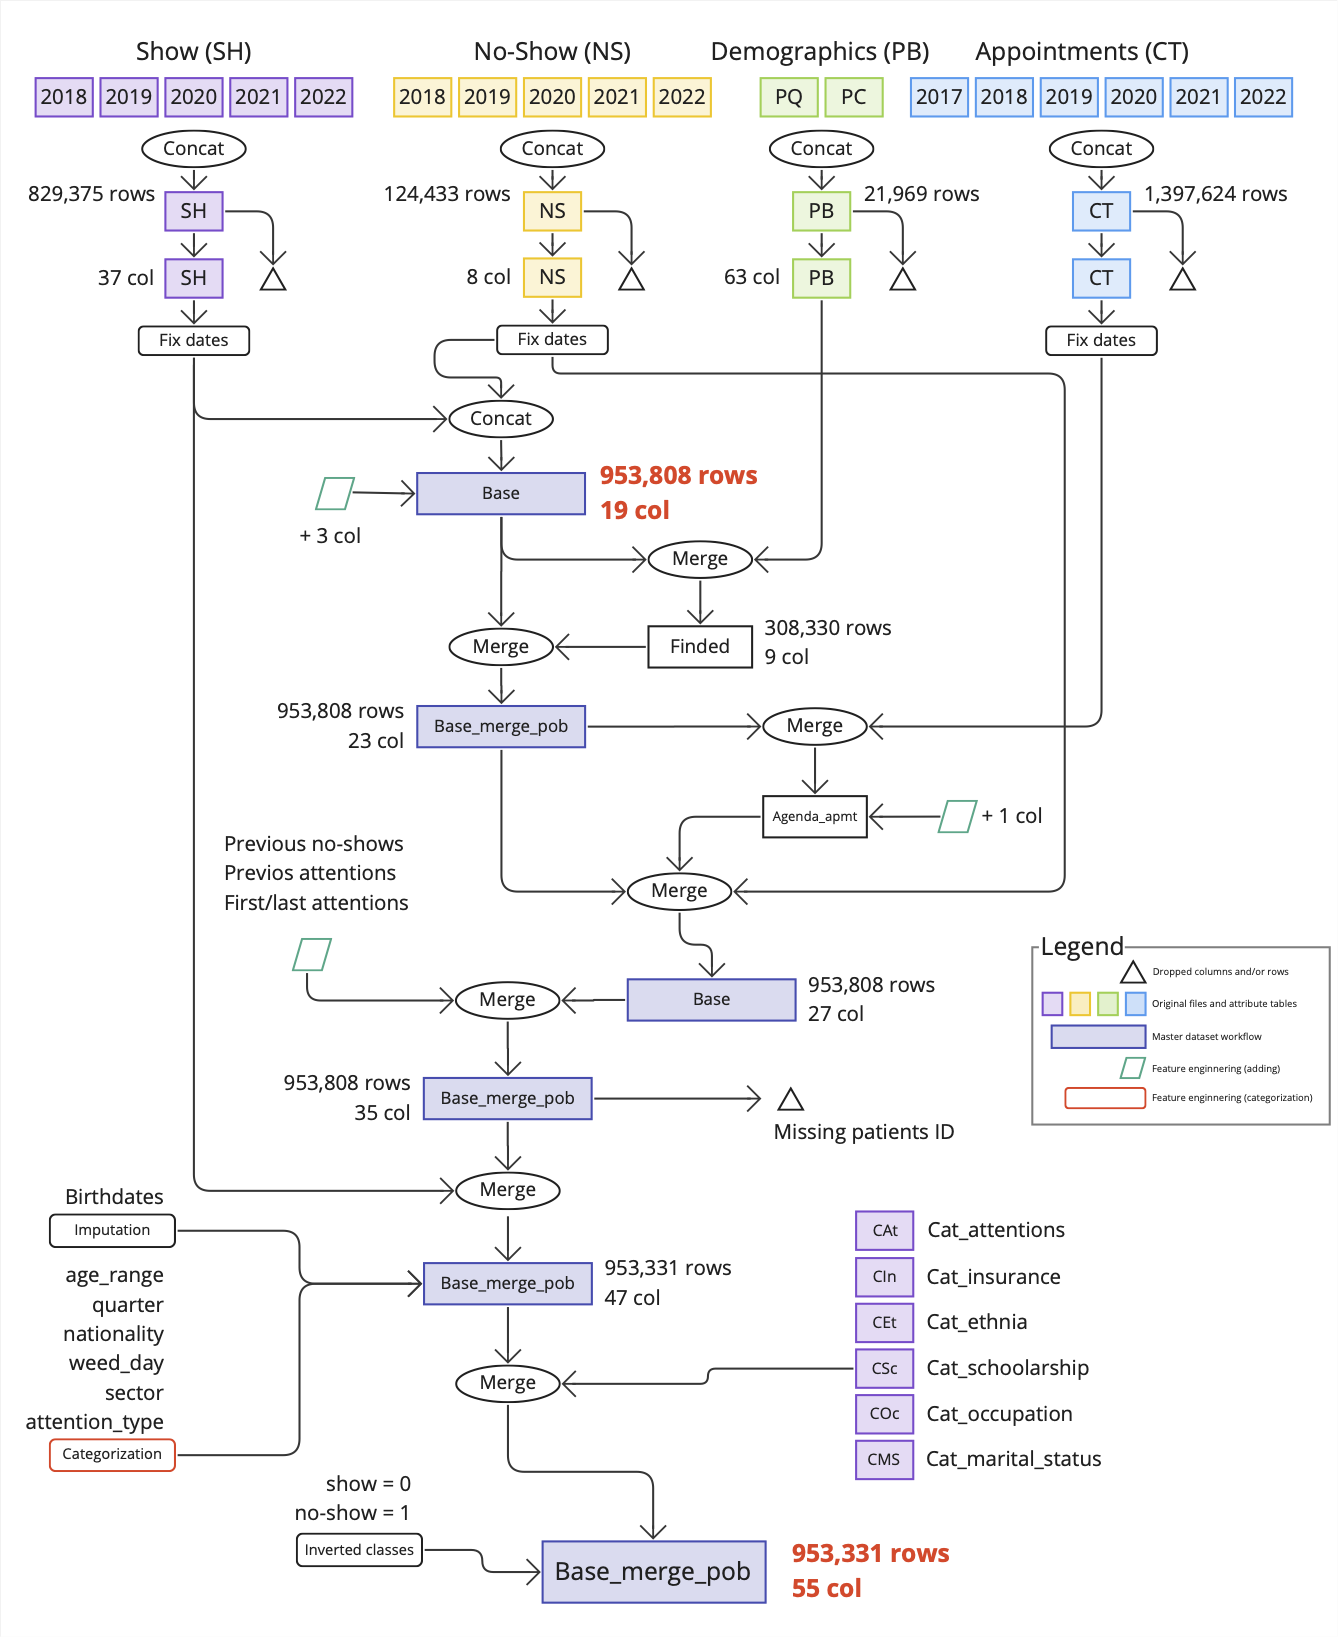
\includegraphics[width=0.9\textwidth]{img/no.show-pre_processing.png}
        \caption{Actual cleaning and pre-processing workflow.}
      \label{fig:pre-processing}
    \end{figure}

\end{appendices}
\end{document}
